% TODO: @lukas this paragraph seems kind of useless, can we think of something better to say?

This project was done by three people: Two students who implemented the tool and their superior. So there had to be a lot of communication. The communication tools were offline meetings, Slack and emails. For filesharing Github is used.

%\paragraph*{Slack} is an web-based instant-messaging-service especially for team-projects. For this Project a channel with two integrations was used. The first integration is the Github integration, with shows all activities on a github repository. The other one is the circlecl integration, which shows the result of the CI-tests.

\subsubsection*{timeline}
From the timeline (Figure \ref{fig:timeline}) can be derived that this project was realized in less then 9 months. The real worktime exposure ratio of the three main-task (reading, programming and writing) differs extremely from the visualized one. In reality we read 50\%, programmed 40\% and wrote 10\% of the worktime.
It is also visible that we didn't manage to complete three milestones in time. This was caused by different circumstances, but we managed to complete the hole project in time cause we adjusted our planing every few weeks.

\begin{figure}[!htb]
	\centering
		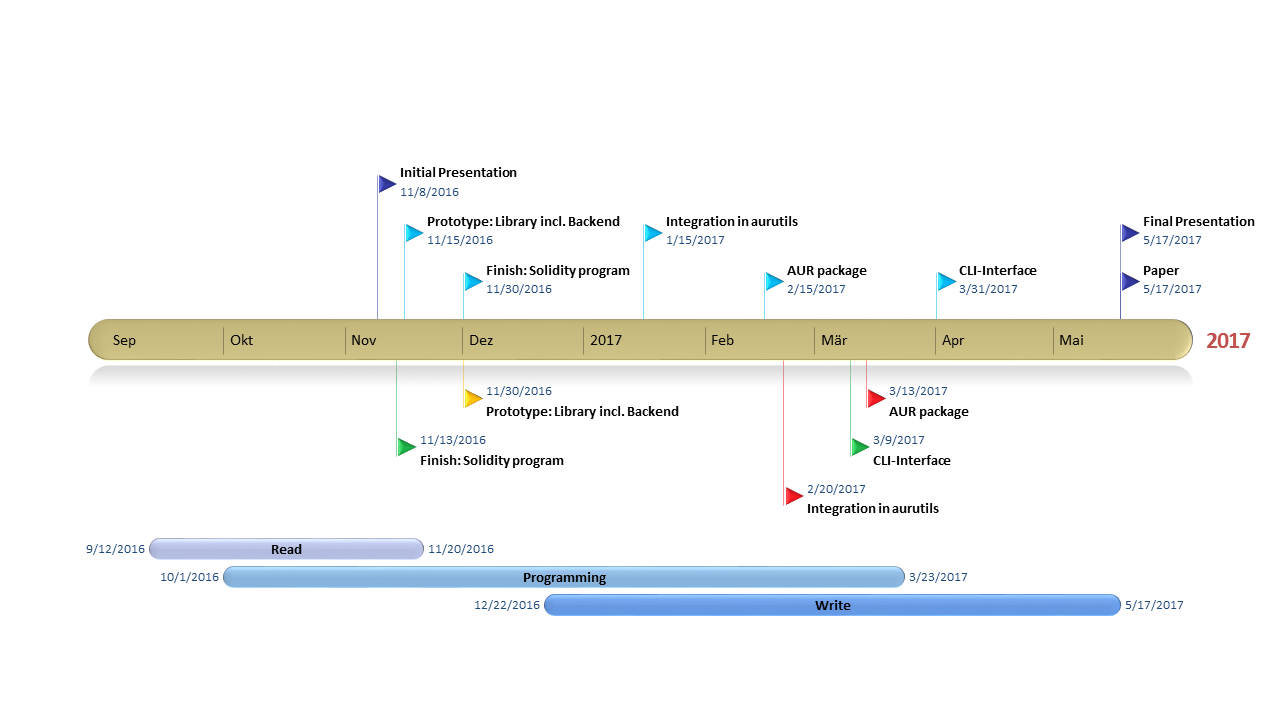
\includegraphics[width=0.7\paperwidth]{timeline}
	\caption{Timeline}
	\label{fig:timeline}
\end{figure}


% Notes:
% TODO: Add refs
